\documentclass[11pt,a4paper]{article}
% =====================================================================
% PLOS NTD revision v3 (page-audit).
% PROVENANCE: This LaTeX manuscript source was reconstructed from the June 26, 2026
% manuscript PDF and user-supplied manuscript text. It is not the original authoring
% source. Revision v3 was derived from the preserved working state of revision v2 after
% a full page-by-page audit of the 17-page review PDF.
% Numbers are reused verbatim from the frozen committed reports (no recomputation).
% Unresolved administrative metadata are tracked in submission_blockers_v3.md, not in
% the manuscript body. Not for submission until the authors confirm those items.
% =====================================================================
\usepackage[utf8]{inputenc}
\usepackage[T1]{fontenc}
\usepackage{lmodern}
\usepackage{amsmath,amsfonts,amssymb}
\usepackage{booktabs}
\usepackage{threeparttable}
\usepackage{geometry}
\usepackage{microtype}
\usepackage{tabularx}
\usepackage{array}
\usepackage{float}
\usepackage{placeins}
\usepackage{pgfplots}
\pgfplotsset{compat=1.18}
% Force fixed-point (non-scientific) y-axis tick labels on all plots.
\pgfplotsset{every axis/.append style={scaled y ticks=false, yticklabel style={/pgf/number format/.cd, fixed, precision=2, /tikz/.cd}}}
\usepackage{tikz}
\usepackage{xcolor}
\usepackage{setspace}
\usepackage[numbers,sort&compress]{natbib}
\usepackage[colorlinks=true,linkcolor=black,citecolor=black,urlcolor=black]{hyperref}
\usepackage{lineno}
\usetikzlibrary{arrows.meta, positioning, shapes.geometric}

% ---- Okabe-Ito colorblind-safe palette (grayscale-legible) ----
\definecolor{okBlue}{RGB}{0,114,178}
\definecolor{okOrange}{RGB}{230,159,0}
\definecolor{okGreen}{RGB}{0,158,115}
\definecolor{okVermillion}{RGB}{213,94,0}
\definecolor{okPurple}{RGB}{204,121,167}
\definecolor{okSky}{RGB}{86,180,233}
\definecolor{okYellow}{RGB}{240,228,66}
\definecolor{okGray}{RGB}{120,120,120}

\geometry{margin=1in}
\doublespacing
% Line numbers disabled per author request (re-enable with \linenumbers for journal review if required).
%\linenumbers

\begin{document}

% =====================================================================
% TITLE PAGE
% =====================================================================
\begin{center}
{\Large \textbf{Benchmarking Climate-Informed Dengue Early Warning Against Recent Surveillance: Calibration and Decision-Curve Evidence from Sri Lanka and Colombia}}\\[1.2em]

Ganesh Shiwakoti\textsuperscript{1,\,$\ast$} and Bhimsen Khadka\textsuperscript{2}\\[0.6em]

\footnotesize
\textsuperscript{1}Department of Mathematics and Statistics, Florida Atlantic University, Boca Raton, Florida, USA\\
\textsuperscript{2}Department of Mathematical Sciences, The University of Texas at Dallas, Richardson, Texas, USA\\[0.3em]
$\ast$\,Corresponding author: ganshiwakoti@gmail.com\\[0.7em]
\textit{Administrative metadata pending --- not for submission.}
\end{center}

\vspace{0.5em}

% =====================================================================
% STRUCTURED ABSTRACT (PLOS NTD: Background / Methodology & Principal
% Findings / Conclusions & Significance; 250-300 words; NO citations)
% =====================================================================
\begin{abstract}
\noindent\textbf{Background.}
Climate-informed dengue early-warning systems are usually judged by discrimination, such as the area under the receiver-operating characteristic curve, and against weak baselines such as seasonal climatology. Public-health deployment, however, depends on whether predicted risks improve calibrated, threshold-based alert decisions beyond the information already available from routine surveillance.

\noindent\textbf{Methodology/Principal Findings.}
We conducted a retrospective decision-evaluation of dengue early-warning models in Sri Lanka (primary, RDHS-week, 2018--2025) and Colombia (external framework replication), comparing a recent-case surveillance baseline (M1) with climate-only, structured-climate, and hybrid climate--surveillance models. Models were evaluated at a four-week horizon by discrimination, calibration, recalibration, and decision-curve net benefit at a primary reference threshold of $p^*=0.30$. In Sri Lanka, recent-case surveillance was hard to beat: climate-only models did not exceed it on net benefit, and the hybrid M5$-$M1 net-benefit estimate was $+0.0081$ (95\% CI $-0.0012$ to $+0.0181$). All models under-predicted in the higher-prevalence test period, but rolling 52-week intercept-only recalibration substantially reduced (without eliminating) calibration-in-the-large error and did not change the ranking. In Colombia, the hybrid M5$-$M1 net-benefit estimate was $+0.0188$ (95\% CI $+0.0117$ to $+0.0260$; $\Delta$AUC $+0.040$), equivalent to approximately 1.9 net true-positive equivalents per 100 municipality-weeks at $p^*=0.30$, or, equivalently, approximately 4.4 fewer false-alert equivalents per 100 --- decision-analytic representations of the same difference, not observed outcomes. Across 1--12-week horizons the increment was approximately flat rather than increasing with lead time. The intervals from the two settings overlap and no cross-country interaction or heterogeneity test was performed, so the settings were not shown to differ.

\noindent\textbf{Conclusions/Significance.}
Climate information is not a standalone replacement for recent dengue surveillance; its operational value is most defensible as a modest hybrid increment whose magnitude and precision varied across the evaluated settings, and which requires local evaluation. Dengue early-warning evaluations should benchmark against recent surveillance and report calibration and decision-curve net benefit alongside discrimination.
\end{abstract}

% =====================================================================
% AUTHOR SUMMARY (150-200 words; nontechnical; first-person; no acronyms)
% =====================================================================
\section*{Author Summary}
Dengue early-warning systems often use weather and climate data to anticipate weeks of elevated dengue activity, and they are usually judged by how well they separate high-risk from low-risk weeks. Here, an alert week was one in which dengue activity exceeded a locally defined historical level, not an official outbreak declaration. Health agencies already track recent dengue case counts, which carry strong short-term information about where cases are rising. We asked a more practical question: does adding climate information improve the alert decisions agencies actually make, beyond what recent case counts already tell them? We evaluated climate-informed dengue models in Sri Lanka and Colombia against a recent-case surveillance benchmark, judging them by whether their predicted risks were well calibrated and improved alert decisions, not only by ranking accuracy. We found that recent surveillance was hard to beat, and climate alone added little. Combining climate with recent cases gave a small improvement whose magnitude and precision varied across the two evaluated datasets, and it did not grow with longer lead times. Because the two datasets were not formally compared, this improvement may be setting-dependent. We suggest climate is more useful as a complement to surveillance than a replacement.

% =====================================================================
% INTRODUCTION
% =====================================================================
\section{Introduction}

Dengue is a major public-health challenge across tropical and subtropical regions, and early-warning systems are widely promoted to anticipate periods of elevated transmission. Transmission depends on mosquito ecology, human susceptibility, movement, public-health control, and environmental conditions, and climate variables such as temperature, humidity, and rainfall influence mosquito abundance, survival, biting, and viral replication, which makes climate-informed early warning conceptually attractive~\cite{Mordecai2017,Huber2018}.

Most dengue early-warning studies evaluate prediction models using discrimination or forecast-accuracy metrics~\cite{Johansson2019,Baharom2022,HussainAlkhateeb2021,Lowe2021}. Discrimination describes whether a model ranks high-risk periods above low-risk periods, but it is incomplete for operational decision-making. A public-health alert system must support threshold-based action, and a model with acceptable discrimination may still be poorly calibrated or may fail to improve net benefit relative to simpler alert strategies. Calibration is therefore central, because decisions depend on predicted probabilities and because calibration can drift when the deployment period differs in baseline incidence from the training period~\cite{VanCalster2019,VanCalster2023,SteyerbergVergouwe2014}.

Decision-curve analysis offers a complementary evaluation of whether a model improves threshold-based decisions~\cite{Vickers2006,Vickers2016,Vickers2019}. Net benefit weighs true-positive gains against the false-positive cost implied by a decision threshold, which connects to cost--loss reasoning in which the threshold encodes the trade-off between unnecessary response and missed elevated transmission~\cite{Murphy1985,Tozan2023}. The relevant comparison, however, is frequently overlooked. A central and demanding benchmark is recent dengue surveillance itself: because incidence is temporally autocorrelated, recent case counts contain strong short-term information, and a climate-informed model that appears useful against a climatological or null baseline may add little beyond information agencies already hold. Operational early-warning frameworks accordingly emphasize recent case activity~\cite{EWARScsd}.

The operational question is therefore not whether climate carries predictive signal for dengue beyond chance, but whether climate adds value beyond recent cases, and whether any such value is visible under calibration and decision-curve evaluation rather than discrimination alone. We address this question with a surveillance-benchmarked, calibration-aware, decision-analytic framework. The primary analysis uses Sri Lanka RDHS-week surveillance linked to climate and population data, with a date-aligned linkage between weekly reports and ISO climate weeks. We apply the same evaluation logic to Colombia as an external framework replication, refitting all models locally rather than transporting coefficients, which lets us distinguish climate-only superiority, no value from climate, and modest, potentially setting-dependent value when climate is integrated with surveillance. We do not propose a new forecasting model or claim methodological novelty for calibration or decision-curve analysis; the contribution is an honest operational evaluation of whether climate-informed dengue early warning improves calibrated, threshold-based decisions beyond routine surveillance.

% =====================================================================
% METHODS
% =====================================================================
\section{Methods}

\subsection{Study design and reporting}
We conducted a retrospective decision-evaluation of dengue early-warning models using weekly surveillance, climate, population, and spatial data. The aim was not to develop a forecasting model but to evaluate whether climate-informed models add operational decision value beyond recent dengue surveillance, judged by discrimination, calibration, time-updated recalibration, and decision-curve net benefit. The primary analysis was Sri Lanka, with one Regional Director of Health Services (RDHS) division and one epidemiological week as the unit. Colombia was a secondary external framework replication using the same evaluation logic with local refitting. Discrimination was treated as secondary to calibration and decision-curve net benefit. Reporting follows an observational-study checklist (STROBE) with a prediction-model reporting and risk-of-bias self-assessment (TRIPOD+AI; PROBAST), provided as Supporting Information~\cite{vonElm2007,Collins2024TRIPODAI,Wolff2019,Moons2019}.

\subsection{Settings and spatial units}
For Sri Lanka the spatial frame contained 26 RDHS units, built from public administrative boundary data~\cite{HDXCODABSriLanka}; 24 corresponded one-to-one with administrative districts, and the Ampara district was split into Ampara and Kalmunai RDHS along divisional-secretariat boundaries. Geometry quality control confirmed all 26 units present, valid non-duplicated geometries, name matching to the surveillance crosswalk, and conservation of the parent district area within projection tolerance. A queen-contiguity adjacency graph (26 nodes, 60 undirected edges, one connected component, no cross-sea links) provided a spatial backbone for sensitivity work. Colombia used the same conceptual ladder with all models refit locally, and is interpreted as external framework replication rather than geographic transport.

\subsection{Surveillance outcomes and alert labels}
For Sri Lanka, current-week dengue case counts were taken from the Weekly Epidemiological Report (WER)~\cite{SriLankaWER}; cumulative counts were used only for quality control. Counts were converted to weekly incidence using annual RDHS population denominators. For Colombia, weekly municipality-level (Admin-2 / GID\_2) dengue counts were obtained from the OpenDengue database (V1.3 Temporal extract)~\cite{Clarke2024OpenDengue,OpenDengue2024}; the data were acquired from the OpenDengue repository rather than directly from the national surveillance system (SIVIGILA), are curated/finalized rather than real-time. The OpenDengue V1.3 release has database coverage through 2023; the Colombia weekly Admin-2 series used here extends through 2022 (test period 2020--2022). The alert label was unit-specific: for each unit the 75th percentile of weekly incidence was estimated from the training period only, and a future week was an alert if its incidence exceeded that threshold. The primary horizon was $h=4$ weeks: for an observation at week $t$, predictors used information through week $t$ and the target was the alert at week $t+4$, constructed by a date-based join (the calendar week beginning 28 days later) rather than a positional shift. A 90th-percentile label was used as a stricter outcome-definition sensitivity, and horizons $h=1,2,8,12$ were used as horizon sensitivities.

\subsection{Population denominators}
Annual RDHS denominators for 2018--2025 were built from WorldPop rasters~\cite{Tatem2017,WorldPop2025} aggregated to the 26 polygons, then district-anchored to the 2024 Sri Lanka Census~\cite{SriLankaCensus2025}. For one-to-one districts, $\mathrm{Pop}_{\mathrm{adj}}(d,y)=\mathrm{Census}_{2024}(d)\times \mathrm{WorldPop}(d,y)/\mathrm{WorldPop}(d,2024)$; the Ampara total was anchored then split between Ampara and Kalmunai by their WorldPop ratio. The 208-record (26 units $\times$ 8 years) table passed checks for completeness, positivity, no extreme year-to-year change, and exact agreement with 2024 census district and national totals. Population was constant within each epidemiological year.

\subsection{Climate exposures and temporal alignment}
Weekly RDHS temperature and humidity were derived from ERA5-Land~\cite{MunozSabater2021,ERA5LandCDS} (mean/min/max two-meter temperature; relative humidity from temperature and dewpoint via the Magnus formula) and precipitation from CHIRPS~\cite{Funk2015,CHIRPS}, aggregated on the frozen 26-RDHS geometry and frozen before outcome modeling. A key linkage issue was that the stored WER week label was the issue number, not the ISO climate week; an audit of WER dates showed the issue number led the ISO surveillance week by approximately one week in most years and by approximately two weeks in 2021 (issue 43 unpublished; issue 53 duplicating issue 52). The primary linkage therefore mapped each issue to its ISO week using reporting-date information; the duplicate was excluded and genuinely missing issues were retained as documented missingness rather than imputed. A naive week-number linkage was retained as a sensitivity. Rows with missing outcome, exposure, or population were excluded from the complete-case frame.

\subsection{Model ladder and fitting}
The ladder distinguished recent-case surveillance, climate-only, and hybrid information. M0 was a seasonal climatological baseline; M1 a recent-case surveillance baseline (recent incidence lags, seasonal harmonics, geographic fixed effects); M2 a climate-only model; M3 a structured climate model (climate, seasonality, geographic fixed effects); M4 a hybrid (recent cases plus weekly climate features); and M5 a hybrid additionally including seasonality and geographic fixed effects. The conceptual M0--M5 labels do not guarantee identical feature implementation across countries, and the implementations differed: in Sri Lanka the hybrid climate component was a Python distributed-lag nonlinear cross-basis (temperature, precipitation, humidity; lags 0--8 weeks; df=3), whereas in Colombia the climate component used linear weekly precipitation and temperature lags (\texttt{precip\_lag0--8}, \texttt{temp\_lag0--8}; humidity was not used in Colombia). Penalty type and tuning also differed by setting. The per-country implementation is detailed in Supporting Information (S5 Table). A canonical R \texttt{dlnm} comparator assessed whether a standard distributed-lag nonlinear specification changed the Sri Lanka climate-only conclusion~\cite{Gasparrini2010,Gasparrini2011}.

Sri Lanka models were fit on 2018--2022 and evaluated on 2023--2025. The held-out test period was not used for model fitting, predictor scaling, penalty selection, or alert-threshold construction. Time-updated recalibration was evaluated sequentially during the test period using only forecast--outcome pairs whose outcomes would have been observed before each prediction time, thereby avoiding look-ahead. The primary logistic models used L2 (ridge) penalization; the regularization strength was selected on the training data only, and convergence and separation were checked against prespecified stop rules (no stop triggered). Recent-case lags used only information available at or before the predictor week, and early-series missing lags used training-period imputation rules. Colombia used the same logic with local data and refitting. Analyses used Python and R~\cite{RCoreTeam2024}; package versions are listed in Supporting Information (S5 Table), with any version not preserved in the reproducibility record marked as such.

\subsection{Calibration and time-updated recalibration}
Calibration was assessed on held-out predictions by calibration-in-the-large (CITL), calibration slope, mean predicted probability, observed prevalence, and Brier score, interpreted jointly with discrimination and net benefit. Because the Sri Lanka test period had higher alert prevalence than training, a time-updated recalibration was applied on the logit of the raw prediction. The primary method was rolling 52-week intercept-only recalibration using only forecast--outcome pairs whose targets were fully observed before the prediction week; rolling 104-week and expanding-window variants, and intercept-plus-slope forms, were also evaluated under prespecified minimum-sample and convergence rules. No fallback was required under the prespecified recalibration rules.

\subsection{Decision-curve analysis and the reference threshold}
For a threshold probability $p^*$, net benefit was
\[
\mathrm{NB}(p^*)=\frac{\mathrm{TP}}{N}-\frac{\mathrm{FP}}{N}\,\frac{p^*}{1-p^*},
\]
with TP and FP the true- and false-positive alerts and $N$ the number of observations; the threshold-probability interpretation follows cost--loss reasoning~\cite{Vickers2006,Murphy1985,Tozan2023}. A model has operational value at $p^*$ if its net benefit exceeds the default alert-all and alert-none strategies. We used $p^*=0.30$ as the \emph{primary reference threshold}. This is not an empirically established public-health threshold; it encodes a particular trade-off between the cost of an unnecessary alert and the loss from a missed alert, and we therefore report net benefit across a threshold grid to show robustness across the evaluated range rather than relying on a single point. Discrimination (AUC, PR-AUC)~\cite{SaitoRehmsmeier2015} was reported but not treated as sufficient evidence of operational value.

\subsection{Uncertainty, multiplicity, and analysis status}
Uncertainty for key contrasts used cluster bootstrap resampling of the spatial unit (RDHS for Sri Lanka, municipality/GID\_2 for Colombia), resampling units with replacement and retaining all weeks within a sampled unit~\cite{CameronGelbachMiller2008}. The common verified principles were percentile intervals from resampling the spatial unit, with degenerate one-class resamples excluded from discrimination summaries and the failure count recorded; the resampling unit, number of replicates, seed, interval method, and failure handling are specified per analysis in Supporting Information (S6 Table), and the main text does not assume a shared protocol across all analyses. The principal estimand was $\Delta\mathrm{NB}(p^*,z)=\mathrm{NB}_{\mathrm{M5}}(p^*\mid z)-\mathrm{NB}_{\mathrm{M1}}(p^*\mid z)$ over the full test set or a regime $z$. Within each setting, $\Delta\mathrm{NB}(\text{M5}-\text{M1})$ at $p^*=0.30$ under the $h=4$, 75th-percentile definition was treated as the primary reference contrast; threshold, horizon, percentile, and regime analyses were secondary or exploratory, with pointwise intervals and no multiplicity adjustment. The Sri Lanka pilot is exploratory/hypothesis-generating because it used a single temporal holdout rather than a rolling-origin and spatial-block design, and some decision-threshold and uncertainty components were documented extensions. Colombia is external framework replication, not external model validation, and surveillance counts are finalized rather than real-time, so results reflect retrospective performance on completed counts. The dated analysis plan and documented addenda are retained in the project repository; no prospective public registration is claimed.

% =====================================================================
% RESULTS
% =====================================================================
\section{Results}

\subsection{Cohort and data alignment}
Each Sri Lanka observation was one RDHS division and one epidemiological week, with the four-week-ahead 75th-percentile alert as the target. Because the WER issue number led the ISO climate week, the primary analysis used the date-aligned linkage. After the primary filter the analysis contained 10{,}705 modelable RDHS-week rows, reduced to 10{,}516 after constructing the four-week-ahead target. Training (2018--2022) had 6{,}590 observations and 1{,}593 alert events; the test period (2023--2025) had 3{,}926 observations and 1{,}321 events. Alert prevalence rose from 24.2\% (training) to 33.6\% (testing), a higher-incidence test period (Fig~\ref{fig:pipeline}).

\begin{figure}[htbp]
\centering
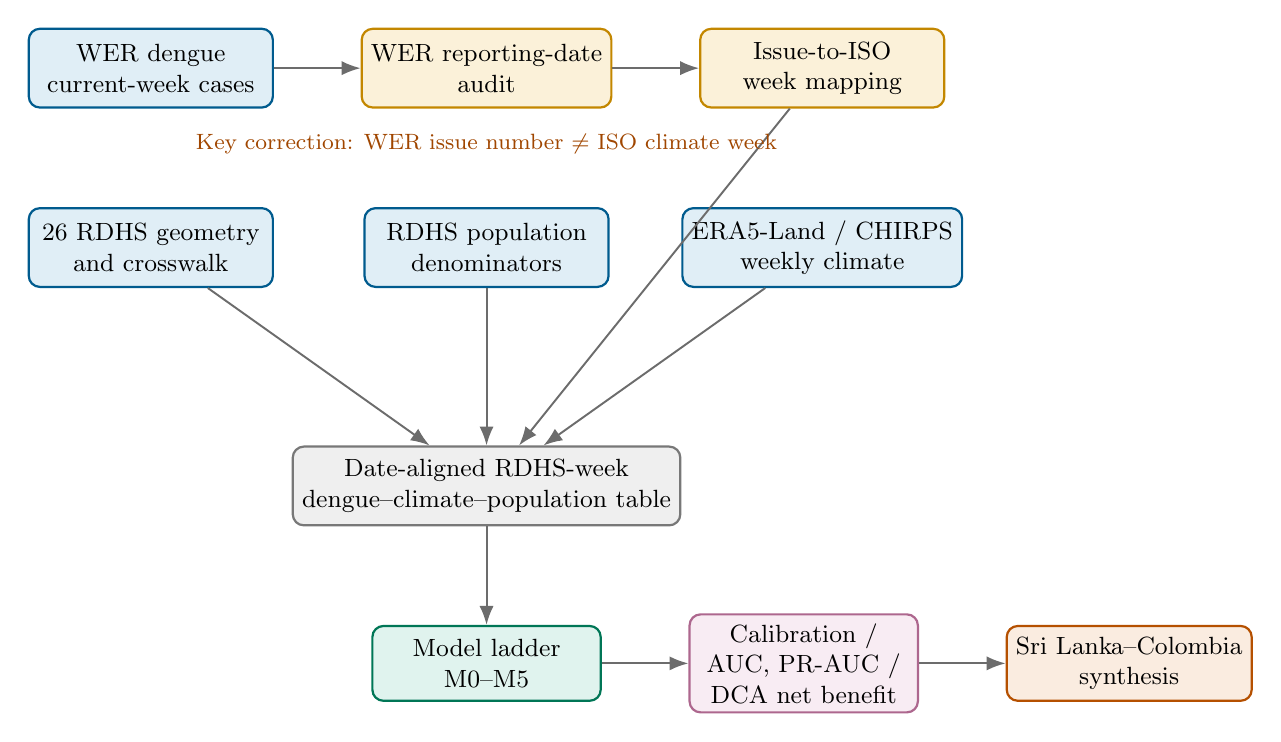
\begin{tikzpicture}[
    node distance=1.25cm and 1.1cm,
    every node/.style={font=\small},
    src/.style   ={rectangle, rounded corners, draw=okBlue!80!black, fill=okBlue!12, line width=0.8pt, align=center, minimum width=3.1cm, minimum height=1.0cm},
    pre/.style   ={rectangle, rounded corners, draw=okOrange!85!black, fill=okOrange!15, line width=0.8pt, align=center, minimum width=3.1cm, minimum height=1.0cm},
    integ/.style ={rectangle, rounded corners, draw=okGray, fill=okGray!12, line width=0.8pt, align=center, minimum width=4.6cm, minimum height=1.0cm},
    mod/.style   ={rectangle, rounded corners, draw=okGreen!75!black, fill=okGreen!12, line width=0.8pt, align=center, minimum width=2.9cm, minimum height=0.95cm},
    evaln/.style ={rectangle, rounded corners, draw=okPurple!85!black, fill=okPurple!14, line width=0.8pt, align=center, minimum width=2.9cm, minimum height=0.95cm},
    outnode/.style={rectangle, rounded corners, draw=okVermillion!85!black, fill=okVermillion!12, line width=0.8pt, align=center, minimum width=2.9cm, minimum height=0.95cm},
    arrow/.style ={-{Latex[length=2.4mm]}, line width=0.7pt, draw=okGray!90!black}
]
\node[src] (wer) {WER dengue\\current-week cases};
\node[pre, right=of wer] (date) {WER reporting-date\\audit};
\node[pre, right=of date] (iso) {Issue-to-ISO\\week mapping};
\node[src, below=of iso] (climate) {ERA5-Land / CHIRPS\\weekly climate};
\node[src, below=of date] (pop) {RDHS population\\denominators};
\node[src, below=of wer] (geom) {26 RDHS geometry\\and crosswalk};
\node[integ, below=2.0cm of pop] (linked) {Date-aligned RDHS-week\\dengue--climate--population table};
\node[mod, below=of linked] (models) {Model ladder\\M0--M5};
\node[evaln, right=of models] (eval) {Calibration /\\AUC, PR-AUC /\\DCA net benefit};
\node[outnode, right=of eval] (synth) {Sri Lanka--Colombia\\synthesis};
\draw[arrow] (wer) -- (date);
\draw[arrow] (date) -- (iso);
\draw[arrow] (iso) -- (linked);
\draw[arrow] (climate) -- (linked);
\draw[arrow] (pop) -- (linked);
\draw[arrow] (geom) -- (linked);
\draw[arrow] (linked) -- (models);
\draw[arrow] (models) -- (eval);
\draw[arrow] (eval) -- (synth);
\node[align=center, font=\footnotesize, text=okVermillion!75!black, below=0.2cm of date]
 {Key correction: WER issue number $\neq$ ISO climate week};
\end{tikzpicture}
\caption{Study pipeline and WER date-alignment rule. Color encodes object category: data sources (blue), preprocessing (orange), the integrated analytic table (gray), model families (green), evaluation (purple), and synthesis output (vermillion). The primary Sri Lanka analysis used a date-derived ISO epidemiological week rather than the stored WER issue number, preventing climate exposures from being joined to dengue outcomes from the wrong calendar week. The palette is colorblind-safe (Okabe--Ito) and legible in grayscale.}
\label{fig:pipeline}
\end{figure}

\subsection{Sri Lanka primary comparison}
Among the initial M0--M3 benchmark comparison, in the held-out 2023--2025 test period the recent-case surveillance model M1 had the highest discrimination, lowest Brier score, and highest net benefit at $p^*=0.30$ (Table~\ref{tab:slprimary}). The climate-only and structured-climate models showed predictive signal but did not exceed M1. At $p^*=0.30$, M1 net benefit was 0.137, versus 0.069 (M2) and 0.078 (M3); alert-all was lower than M1 and alert-none was zero. Decision value was threshold-dependent (Table~\ref{tab:slthresh}, Fig~\ref{fig:sldca}): at low thresholds alert-all was competitive, as expected when the threshold lies well below test prevalence, while across the mid-to-high range M1 was consistently highest among M0--M3.

\begin{table}[htbp]
\centering
\caption{Initial Sri Lanka M0--M3 benchmark comparison ($h=4$, RDHS 75th-percentile alert label, 2023--2025 test period). Hybrid models M4--M5 are reported separately.}
\label{tab:slprimary}
\begin{threeparttable}\footnotesize
\setlength{\tabcolsep}{3.6pt}
\begin{tabular}{llrrrrrrrr}
\toprule
Model & Description & AUC & PR-AUC & Brier & CITL & Slope & Mean pred. & Obs. & NB$_{0.30}$ \\
\midrule
M0 & Seasonal climatology & 0.629 & 0.459 & 0.222 & +0.530 & 0.664 & 0.238 & 0.336 & 0.084 \\
M1 & Recent-case surveillance & 0.752 & 0.652 & 0.191 & +0.513 & 1.246 & 0.246 & 0.336 & 0.137 \\
M2 & Climate-only & 0.643 & 0.460 & 0.220 & +0.479 & 1.027 & 0.243 & 0.336 & 0.069 \\
M3 & Climate + season + RDHS FE & 0.652 & 0.476 & 0.220 & +0.596 & 0.738 & 0.229 & 0.336 & 0.078 \\
\bottomrule
\end{tabular}
\begin{tablenotes}\footnotesize
\item CITL, calibration-in-the-large; NB$_{0.30}$, net benefit at the primary reference threshold $p^*=0.30$.
\end{tablenotes}
\end{threeparttable}
\end{table}

\begin{table}[htbp]
\centering
\caption{Sri Lanka net benefit at representative decision thresholds.}
\label{tab:slthresh}
\small
\begin{tabular}{rrrrrrr}
\toprule
Threshold $p^*$ & Alert-all & Alert-none & M0 & M1 & M2 & M3 \\
\midrule
0.20 & 0.171 & 0 & 0.161 & 0.185 & 0.164 & 0.147 \\
0.30 & 0.052 & 0 & 0.084 & 0.137 & 0.069 & 0.078 \\
0.34 & $-0.005$ & 0 & 0.059 & 0.111 & 0.032 & 0.060 \\
0.40 & $-0.106$ & 0 & 0.025 & 0.083 & 0.012 & 0.039 \\
\bottomrule
\end{tabular}
\end{table}

\begin{figure}[htbp]
\centering
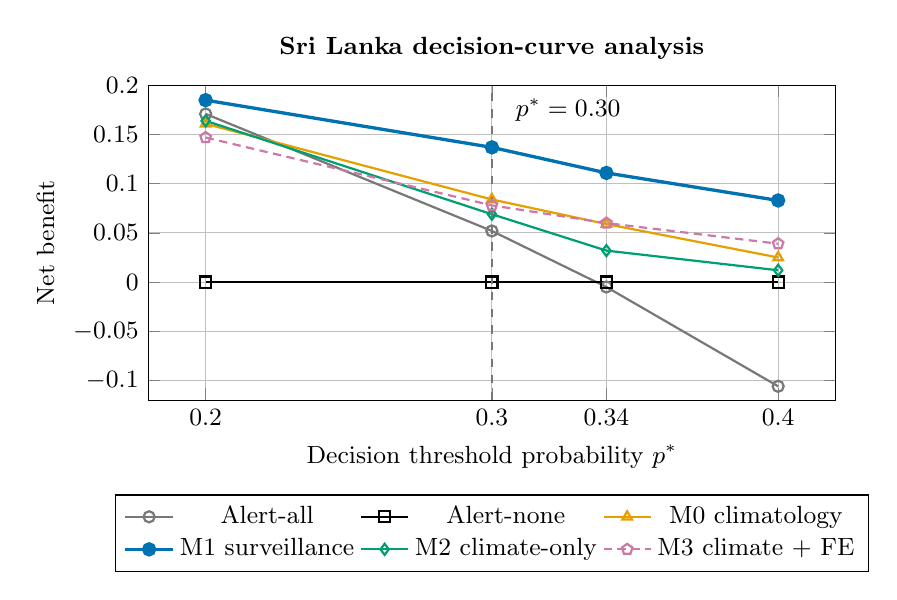
\begin{tikzpicture}
\begin{axis}[
    width=0.85\textwidth, height=0.46\textwidth,
    xlabel={Decision threshold probability $p^*$}, ylabel={Net benefit},
    xmin=0.18, xmax=0.42, ymin=-0.12, ymax=0.20,
    xtick={0.20,0.30,0.34,0.40}, ytick={-0.10,-0.05,0,0.05,0.10,0.15,0.20},
    grid=both, tick label style={font=\small}, label style={font=\small},
    legend style={at={(0.5,-0.30)}, anchor=north, legend columns=3, font=\small},
    title={Sri Lanka decision-curve analysis}, title style={font=\small\bfseries}]
\addplot+[mark=o, thick, color=okGray] coordinates {(0.20,0.171)(0.30,0.052)(0.34,-0.005)(0.40,-0.106)}; \addlegendentry{Alert-all}
\addplot+[mark=square, thick, color=black] coordinates {(0.20,0)(0.30,0)(0.34,0)(0.40,0)}; \addlegendentry{Alert-none}
\addplot+[mark=triangle, thick, color=okOrange] coordinates {(0.20,0.161)(0.30,0.084)(0.34,0.059)(0.40,0.025)}; \addlegendentry{M0 climatology}
\addplot+[mark=*, very thick, color=okBlue] coordinates {(0.20,0.185)(0.30,0.137)(0.34,0.111)(0.40,0.083)}; \addlegendentry{M1 surveillance}
\addplot+[mark=diamond, thick, color=okGreen] coordinates {(0.20,0.164)(0.30,0.069)(0.34,0.032)(0.40,0.012)}; \addlegendentry{M2 climate-only}
\addplot+[mark=pentagon, thick, color=okPurple] coordinates {(0.20,0.147)(0.30,0.078)(0.34,0.060)(0.40,0.039)}; \addlegendentry{M3 climate + FE}
\addplot[dashed, thick, color=okGray] coordinates {(0.30,-0.12)(0.30,0.20)};
\node[anchor=west, font=\small] at (axis cs:0.305,0.175) {$p^*=0.30$};
\end{axis}
\end{tikzpicture}
\caption{Sri Lanka net benefit at representative decision thresholds ($h=4$, 75th-percentile label). Points are net benefit at four representative thresholds (Table~\ref{tab:slthresh}); line segments connect them and do not represent a recomputed continuous grid. The recent-case surveillance model (M1) had the highest net benefit at $p^*=0.30$ and across the mid-to-high range (full $p^*$ grid in Methods/Supporting Information). Colorblind-safe (Okabe--Ito) palette.}
\label{fig:sldca}
\end{figure}

\subsection{Calibration and recalibration}
All M0--M3 models in the initial comparison under-predicted in the test period (CITL $+0.530$ M0, $+0.513$ M1, $+0.479$ M2, $+0.596$ M3; mean predicted $\approx$0.23--0.25 against observed prevalence 0.336), consistent with the 24.2\%$\rightarrow$33.6\% training-to-test prevalence shift. Rolling 52-week intercept-only recalibration substantially reduced calibration-in-the-large error for all models, leaving residual CITL of $+0.029$ (M0), $+0.020$ (M1), $+0.046$ (M2), and $+0.087$ (M3) (Table~\ref{tab:recal}), and outperformed expanding-window recalibration, which under-corrected. Intercept-only recalibration addresses average under- or over-prediction but does not by itself correct calibration slope or nonlinear miscalibration, so it does not imply perfect calibration; for example, M3's residual CITL was $+0.087$. No recalibration fallbacks occurred in the evaluated rolling-recalibration workflow. Recalibration did not change the model ranking: across the evaluated recalibration methods M1 net benefit at $p^*=0.30$ ranged 0.124--0.142 while the maximum climate-model net benefit was approximately 0.085, so reducing calibration error did not make climate-only models exceed surveillance.

\begin{table}[htbp]
\centering
\caption{Calibration-in-the-large before and after time-updated recalibration.}
\label{tab:recal}
\small
\begin{tabular}{lrrrr}
\toprule
Model & Raw CITL & Rolling-52 & Rolling-104 & Expanding \\
\midrule
M0 & +0.530 & +0.029 & +0.137 & +0.338 \\
M1 & +0.513 & +0.020 & +0.111 & +0.325 \\
M2 & +0.479 & +0.046 & +0.155 & +0.314 \\
M3 & +0.596 & +0.087 & +0.204 & +0.394 \\
\bottomrule
\end{tabular}
\end{table}

\subsection{Sri Lanka structured-climate and hybrid results}
A canonical R \texttt{dlnm} comparator differed from the Python distributed-lag approximation by approximately zero ($\Delta$AUC and $\Delta$NB at $p^*=0.30$ near zero, with 95\% CIs that included zero) and improved over simple climate models but did not exceed M1: at $p^*=0.30$, M1 net benefit was 0.137 versus 0.112 (canonical R DLNM), with $\Delta$AUC $-0.038$ (95\% CI $-0.066$ to $-0.008$) and $\Delta$NB $-0.025$ (95\% CI $-0.041$ to $-0.006$) (Table~\ref{tab:dlnmhybrid}). The hybrid models improved some measures relative to M1; M5 reached AUC 0.772, PR-AUC 0.667, Brier 0.180, and net benefit 0.145 at $p^*=0.30$ (M1: 0.752, 0.652, 0.191, 0.137). The M5$-$M1 net-benefit estimate was $+0.0081$ (95\% CI $-0.0012$ to $+0.0181$): M5 had higher discrimination and a higher net-benefit point estimate than M1 (Table~\ref{tab:dlnmhybrid}; see the cross-setting summary).

\begin{table}[htbp]
\centering
\caption{Sri Lanka canonical DLNM and hybrid comparison (test period, $h=4$, 75th-percentile label).}
\label{tab:dlnmhybrid}
\small
\begin{tabular}{lrrrr}
\toprule
Model & AUC & NB$_{0.20}$ & NB$_{0.30}$ & NB$_{0.40}$ \\
\midrule
M1 recent-case surveillance & 0.752 & 0.185 & 0.137 & 0.083 \\
M2 climate-only & 0.643 & 0.164 & 0.069 & 0.012 \\
M3 climate + season/RDHS & 0.652 & 0.147 & 0.078 & 0.039 \\
Python DLNM-style climate & 0.714 & 0.179 & 0.111 & 0.057 \\
Canonical R DLNM climate & 0.714 & 0.181 & 0.112 & 0.053 \\
M5 hybrid reference & 0.772 & 0.194 & 0.145 & 0.107 \\
\bottomrule
\end{tabular}
\end{table}

\subsection{Colombia external framework replication}
The Colombia primary $h=4$ analysis used a common-complete M1--M5 row set with 13{,}361 test observations and test prevalence 0.375; the split was training 2006--2017, validation 2018--2019, and test 2020--2022. As in Sri Lanka, climate-only models were weak (M2 AUC 0.556, M3 0.564) relative to M1 (AUC 0.685). The hybrid had a higher net-benefit point estimate than M1: M5 AUC 0.726 and net benefit 0.136 at $p^*=0.30$ versus M1 0.685 and 0.117, with municipality-cluster bootstrap $\Delta$AUC $+0.040$ (95\% CI $+0.024$ to $+0.058$) and $\Delta$NB at $p^*=0.30$ $+0.0188$ (95\% CI $+0.0117$ to $+0.0260$) (Table~\ref{tab:colombia}, Fig~\ref{fig:colombia}). At $p^*=0.30$, the $\Delta$NB of $+0.0188$ corresponds to approximately 1.9 additional net true-positive equivalents per 100 municipality-weeks. Equivalently---rather than additionally---holding true-positive detections fixed, it corresponds to approximately 4.4 fewer false-alert equivalents per 100 municipality-weeks, with an approximate interval of 2.7 to 6.1 fewer per 100. These are alternative decision-analytic representations of the same net-benefit difference, not observed numbers of outbreaks detected, alerts prevented, cases prevented, or lives saved. In the larger secondary climate-only row set, M2 and M3 net benefit was approximately 0.001 (AUC $\approx$0.532 and 0.546), indicating that climate-only weakness was not an artifact of the common-complete row set; the two row sets are not combined in a single table. The Colombia test period (2020--2022) includes the COVID-19-era years 2020--2021, and test-period predictions exceeded observed prevalence; the within-test M5-versus-M1 contrast is reported with that limitation.

\begin{table}[htbp]
\centering
\caption{Colombia $h=4$ primary common-complete test performance (external framework replication). Net benefit at $p^*=0.30$ (test prevalence 0.375); alert-all reference $\approx$0.107, alert-none $0$.}
\label{tab:colombia}
\small
\begin{tabular}{llrr}
\toprule
Model & Description & AUC & NB$_{0.30}$ \\
\midrule
M0 & Seasonal climatology & 0.513 & 0.108 \\
M1 & Recent-case surveillance & 0.685 & 0.117 \\
M2 & Climate-only & 0.556 & 0.108 \\
M3 & Climate + seasonality + dept. FE & 0.564 & 0.108 \\
M4 & Hybrid without full fixed effects & 0.699 & 0.129 \\
M5 & Hybrid climate + surveillance & 0.726 & 0.136 \\
\midrule
\multicolumn{2}{l}{Alert-all reference} & --- & $\approx$0.107 \\
\bottomrule
\end{tabular}
\end{table}

\noindent In the primary common-complete analysis, M2 and M3 had net benefit close to alert-all ($\approx$0.107) and below M1. Separately, in the larger secondary climate-only row set, M2 and M3 net benefit was approximately 0.001; the two analyses use different denominators and are not combined.

\begin{figure}[htbp]
\centering
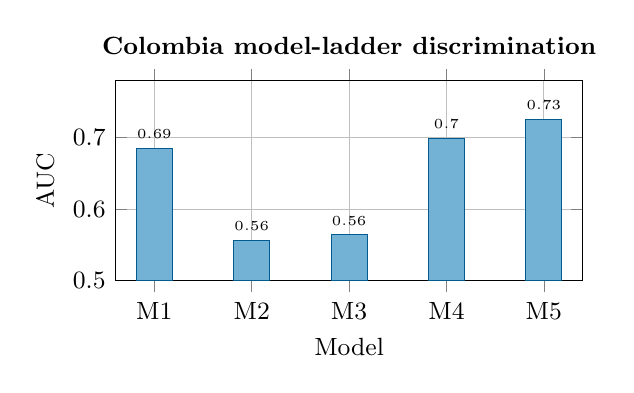
\begin{tikzpicture}
\begin{axis}[
    width=0.62\textwidth, height=0.34\textwidth, ybar, bar width=13pt,
    symbolic x coords={M1,M2,M3,M4,M5}, xtick=data, ymin=0.50, ymax=0.78,
    ylabel={AUC}, xlabel={Model}, grid=both,
    tick label style={font=\small}, label style={font=\small},
    title={Colombia model-ladder discrimination}, title style={font=\small\bfseries},
    nodes near coords, every node near coord/.append style={font=\tiny}]
\addplot[fill=okBlue!55, draw=okBlue!80!black] coordinates {(M1,0.685)(M2,0.556)(M3,0.564)(M4,0.699)(M5,0.726)};
\end{axis}
\end{tikzpicture}
\caption{Colombia model-ladder discrimination. Climate-only models (M2, M3) were weak relative to recent-case surveillance (M1); the hybrid model (M5) had the highest AUC and a higher net-benefit point estimate than M1 ($\Delta$NB $+0.0188$ at $p^*=0.30$; municipality-cluster bootstrap 95\% CI $+0.0117$ to $+0.0260$). Net-benefit values are in Table~\ref{tab:colombia}. Colorblind-safe palette.}
\label{fig:colombia}
\end{figure}

\subsection{Horizon result}
Across the tested Colombia horizons, the M5$-$M1 net-benefit increment was approximately flat rather than increasing with lead time: $\Delta$NB(M5$-$M1) was approximately $+0.015$ to $+0.019$ across $h=1$--8 and approximately $+0.014$ at $h=12$, while $\Delta$AUC fell from approximately $+0.040$ ($h\le4$) to approximately $+0.024$ ($h=12$). In Sri Lanka, the recent-surveillance baseline (M1) retained the highest net benefit at $p^*=0.30$ across the evaluated label--horizon cells; M1 discrimination declined with horizon (AUC 0.843, 0.810, 0.751, 0.679, 0.646 at $h=1,2,4,8,12$ for the 75th-percentile label), with climate models narrowing the discrimination gap at long horizons as M1's own discrimination decayed, without overturning the net-benefit result. The Sri Lanka and Colombia horizon analyses estimate related but not identical quantities. Together, these findings provided no evidence that climate delivered increasing decision value over the tested 1--12-week range.

\subsection{Threshold and stricter-outcome robustness}
In Sri Lanka, a secondary targeted-value analysis across train-defined regimes found the all-test $\Delta$NB(M5$-$M1) at $p^*=0.30$ was $+0.0081$ (95\% CI $-0.0012$ to $+0.0181$); the regime estimates were small with wide, pointwise, multiplicity-unadjusted intervals, and the largest regime estimate (high-incidence $\times$ strong-autocorrelation, $+0.0202$, 95\% CI $+0.0038$ to $+0.0370$) rested on only eight clusters and was treated as underpowered and hypothesis-generating. At $p^*=0.40$ the overall $\Delta$NB was $+0.0241$, a threshold-dependent secondary observation rather than a primary result; intervals across the threshold and percentile grids are pointwise and unadjusted for multiplicity. In Colombia, the secondary stricter exceedance-threshold sensitivity (training-referenced 75th/80th/90th-percentile labels) gave $\Delta$NB(M5$-$M1) at $p^*=0.30$ of $+0.0188$, $+0.0157$, and $+0.0092$, with a diminishing estimate at the 90th percentile (lower confidence limit near zero). Even at the 90th-percentile definition the test-period prevalence of elevated-activity weeks remained approximately 23.5\%, so these are not evidence for rare-epidemic prediction. The 75th-percentile $h=4$ contrast remains the primary analysis. Under the 75th-percentile exceedance-threshold definition the Colombia increment corresponds to approximately 1.9 net true-positive equivalents per 100 municipality-weeks at $p^*=0.30$ (equivalently, not additionally, approximately 4.4 fewer false-alert equivalents per 100): alternative rescalings of the same $\Delta$NB.

\subsection{Cross-setting synthesis}
The Sri Lanka and Colombia hybrid estimates are shown side by side in Table~\ref{tab:crosssetting}. In Sri Lanka, the M5$-$M1 net-benefit estimate was $+0.0081$, with a 95\% CI from $-0.0012$ to $+0.0181$. In Colombia, the corresponding estimate was $+0.0188$, with a 95\% CI from $+0.0117$ to $+0.0260$. The intervals overlap, and no cross-country interaction or heterogeneity test was designed or performed. These results therefore do not establish a difference between settings. Recent surveillance was a strong benchmark in both settings; climate-only models added limited decision value in both; and the hybrid increment was modest and varied in magnitude and precision across the evaluated settings.

\begin{table}[htbp]
\centering
\caption{Cross-setting hybrid increment, $\Delta$NB(M5$-$M1) at $p^*=0.30$ (primary $h=4$, 75th-percentile label). 95\% CIs are percentile bootstrap and pointwise. The intervals overlap, and no cross-country interaction or heterogeneity test was performed; the estimates do not establish a difference between settings.}
\label{tab:crosssetting}
\small
\begin{tabular}{lrr}
\toprule
Setting & $\Delta$NB(M5$-$M1) & 95\% CI \\
\midrule
Sri Lanka (RDHS-cluster bootstrap, all-test) & +0.0081 & $-0.0012$ to $+0.0181$ \\
Colombia (municipality-cluster bootstrap) & +0.0188 & $+0.0117$ to $+0.0260$ \\
\bottomrule
\end{tabular}
\end{table}

% =====================================================================
% DISCUSSION
% =====================================================================
\section{Discussion}

The principal lesson is methodological: climate-informed dengue early-warning models should be evaluated against recent surveillance and judged using calibration and decision-curve net benefit, not discrimination alone. Under that standard, recent surveillance was a strong benchmark in both settings. Climate-only models added limited decision value, while hybrid models showed a modest incremental signal whose magnitude and precision varied across the evaluated settings and which did not increase across the 1--12-week horizons. Formal between-country heterogeneity was not tested.

Climate-only weakness should not be read as climate being irrelevant to transmission. Recent case counts already summarize upstream processes, including climate effects, so over short-to-medium horizons a recent-case baseline is a demanding but appropriate comparator, and even a canonical distributed-lag nonlinear climate model did not exceed it at the primary threshold. The hybrid results are the key nuance: in Sri Lanka the M5$-$M1 net-benefit estimate was $+0.0081$ (95\% CI $-0.0012$ to $+0.0181$), with higher discrimination and a higher net-benefit point estimate than M1, whereas in Colombia the estimate was $+0.0188$ (95\% CI $+0.0117$ to $+0.0260$). The intervals overlap and no between-country heterogeneity test was performed, so the two settings are best read as complementary rather than contradictory and do not establish a difference: climate value may be conditional on setting, surveillance dynamics, and outcome and threshold definitions, and is most defensible as an incremental signal within a hybrid system that requires local evaluation. The operational meaning of the Colombia increment is small. At $p^*=0.30$, the $\Delta$NB of $+0.0188$ corresponds to approximately 1.9 additional net true-positive equivalents per 100 municipality-weeks; equivalently---rather than additionally---holding true-positive detections fixed, it corresponds to approximately 4.4 fewer false-alert equivalents per 100 municipality-weeks (approximate interval 2.7 to 6.1 fewer per 100). These are alternative decision-analytic representations of the same net-benefit difference, not observed numbers of outbreaks detected, alerts prevented, cases prevented, or lives saved.

Two practical evaluation lessons deserve emphasis. First, the date-aligned WER-to-ISO linkage mattered: a naive week-number join would have misaligned climate exposure and dengue outcomes by one to two weeks, which can bias conclusions about lagged climate signal. Second, decision-curve net benefit and calibration revealed patterns that discrimination alone would obscure. Calibration drift was substantial in the test period. Rolling 52-week intercept-only recalibration reduced, but did not eliminate, average miscalibration (for example, M3 residual calibration-in-the-large was $+0.087$). It did not correct calibration slope or nonlinear miscalibration and did not change the model ranking. These patterns argue for ongoing calibration monitoring in any operational use rather than a one-time check.

Several limitations bound these conclusions. The study was retrospective, used finalized rather than real-time surveillance counts, and did not simulate reporting delay; under real-time conditions the recent-case signal that M1 depends on could be degraded, and the direction and magnitude of any change in the relative net benefit of the models cannot be determined from these data. The Colombia test period was 2020--2022 and therefore includes the COVID-19-era years 2020--2021; finalized (rather than real-time) reporting and pandemic-era disruption may affect absolute calibration and comparative performance, and a pandemic-period exclusion analysis was not performed in the current study, so its effect on the M5$-$M1 contrast cannot be inferred. We do not treat the current estimate as a lower bound. Alert labels were percentile (exceedance) thresholds rather than official outbreak declarations, the primary Sri Lanka design used a single temporal holdout rather than a rolling-origin and spatial-block design, climate exposures were aggregated to administrative units (raising change-of-support and modifiable-areal-unit concerns), and the two-country panel is imbalanced. Colombia is external framework replication, not external model validation, so the findings do not establish that coefficients or thresholds transport to other settings, and we make no claim of deployment readiness, transportability, causal climate effects, cost-effectiveness, rare-epidemic prediction, or universal hybrid benefit. Future work should evaluate the framework prospectively under real-time reporting and connect decision thresholds to explicit costs and losses. Mechanistically motivated climate--transmission modeling would require additional serotype, immunity, entomological, mobility, intervention, and reporting-process data and is reserved for separate work.

In summary, recent dengue surveillance is a strong operational benchmark, climate-only models add limited standalone decision value, and climate may add a modest increment within hybrid systems whose magnitude and precision varied across the evaluated settings. Operational evaluations should report calibration and decision-curve net benefit against recent-surveillance baselines before claims of climate-informed value are made.

% =====================================================================
% DECLARATIONS (placeholders; mirror the standalone draft files)
% =====================================================================
\section*{Declarations}
\textbf{Ethics.} The study used aggregate, publicly accessible surveillance data. A formal institutional determination is pending author/institutional confirmation.\\
\textbf{Data and code availability.} Public source datasets (OpenDengue, CHIRPS, ERA5-Land, WorldPop, WER) are cited. Repository and archival details (repository URL, persistent identifier, license) are pending author confirmation.\\
\textbf{Funding.} Pending author confirmation.\\
\textbf{Competing interests.} Pending author confirmation.\\
\textbf{Author contributions.} Pending author confirmation.\\
\textbf{Acknowledgments.} Pending author confirmation.\\
\textbf{Use of AI assistance.} During preparation of this study, the authors used Anthropic Claude through the Claude Code interface under author supervision to assist with drafting and reviewing analysis code, executing prespecified computational workflows, organizing and checking outputs against frozen analysis reports, auditing references, preparing documentation, and editing manuscript language and structure. The authors determined the study questions and analysis decisions, reviewed the code and outputs, independently checked the reported results and citations, and take full responsibility for the accuracy and integrity of the work. The AI system was not listed as an author and did not independently make final scientific or publication decisions.

% =====================================================================
% REFERENCES (Vancouver numbered)
% =====================================================================
\bibliographystyle{unsrtnat}
\bibliography{references_v3}

% =====================================================================
% SUPPORTING INFORMATION CAPTIONS (after References, standard order)
% =====================================================================
\section*{Supporting information}
\noindent Draft/internal Supporting Information items are prepared in the project repository; completed checklists are pending author confirmation (see submission blockers).\\[0.3em]
\noindent\textbf{S1 Checklist.} STROBE checklist for observational studies (draft).\\
\textbf{S2 Checklist.} TRIPOD+AI reporting checklist for prediction models (draft).\\
\textbf{S3 Table.} PROBAST risk-of-bias domain assessment (draft).\\
\textbf{S4 Text.} Analysis-plan and addendum chronology (prespecified vs documented extensions).\\
\textbf{S5 Table.} Per-country M0--M5 model specification (feature lists, recent-case lags, climate variables/lags, seasonality, geographic fixed effects, penalty and tuning), events-per-variable, and software versions.\\
\textbf{S6 Table.} Per-analysis bootstrap protocol (resampling unit, $B$, seed, interval method, degenerate-resample handling, failure count, pointwise/simultaneous and multiplicity status).\\
\textbf{S7 Table.} Sri Lanka sensitivity grid (linkage, climate lag, late-2021 anomaly).\\
\textbf{S8 Table.} Sri Lanka targeted-value regime analysis.\\
\textbf{S9 Table.} Colombia exceedance-threshold (75th/80th/90th) and horizon sensitivity.\\
\textbf{S10 Text.} Reproducibility artifact inventory and checksums.

\end{document}
